\textbf{COLUNI 2019 -- Questão 30}\par\medskip A figura a seguir representa uma flor hermafrodita e suas estruturas principais que estão numeradas:

\par

% COLUNI-AUTO-FIGURES-BEGIN
\begin{figure}[htbp]
\centering
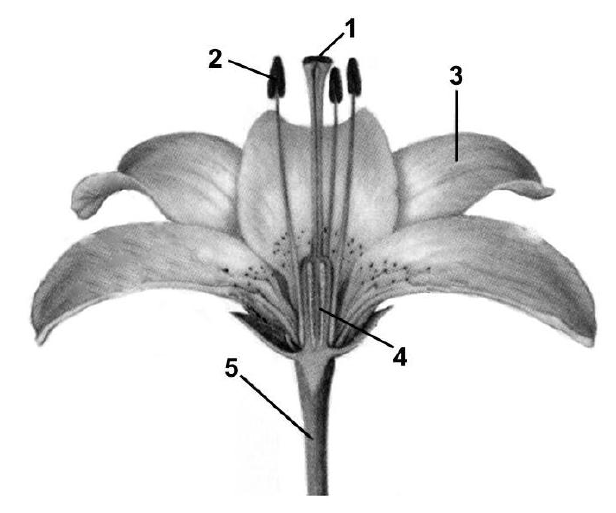
\includegraphics[width=0.95\linewidth]{static/simulados/coluni/figuras/2019/questao-30/figura-1.png}
\end{figure}
% COLUNI-AUTO-FIGURES-END

(CAMPBELL, Neil. A. et al. \textbf{Biology: concepts \& connections}. Menlo Park, Calif: Benjamim Cummings, 1997. Adaptado.)

\par

Leia as seguintes afirmativas sobre as estruturas dessa flor:

\par

I. O grão de pólen é produzido na estrutura 1 e transportado para a estrutura 2 durante a polinização.

II. Os polinizadores, como insetos e aves, são atraídos pela estrutura 3.

III. Após a fecundação, o fruto será originado na estrutura 5.

IV. A estrutura que origina a semente está contida na estrutura 4.

\par

Está CORRETO o que se afirma apenas em:

\par

\begin{enumerate}
\item II e IV.
\item I e II.
\item II, III e IV.
\item I e III.
\end{enumerate}


